%!Mode:: "TeX:UTF-8"
%!TEX program = xelatex
%!TEX TS-program = xelatex
%!TEX encoding = UTF-8 Unicode
%
% Author: Rickjin (ZhihuiJin@gmail.com)
% Author: Leijun  (leijun00@gmail.com)

\chapter{财主的金钱观}

上一章我们讲到 $e$ 是 $(1+ 1/n)^n$ 在 $n$ 趋向于无穷大时的极限,但是这个
极限代表什么意思呢?看上去只是一个干巴巴的数学式子。其实这个极限和我们的日常生
活有很紧密的关系。大家都知道,钱是我们日常生活中非常重要的东西,有钱能使鬼推磨
,没钱寸步难行。其实 $e$ 和钱有着非常紧密的联系,我们从一个故事说起。
\footnote{
故事纯属虚构,如有雷同,实属巧合。
}

\section{财主与打工仔的故事}
在十七世纪欧洲瑞士有个大财主叫雅克比·伯努利,这个财主相当有钱。有钱人挣钱的方
式就是钱生钱,把钱借出去,然后再加倍收回来,这样钱就像滚雪球一样越来越多。有一
天一个没钱的打工仔找到了伯努利老爷,想找伯努利老爷借钱去做点小本生意,伯努利老
爷很爽快的答应了。但是伯努利老爷告诉打工仔,说他借钱年利率很高,高达百分之百。
打工仔虽然很不情愿,但也没别的办法,咬了咬牙,借了一块钱并签字画押,答应一年之
后连本带利一起还回来。一年过去了,打工仔的生意一帆风顺,这时候他找到伯努利老爷
还钱,于是出现了如下的对话。

\begin{figure}[htbp]
\centering

\includegraphics[width=0.7\linewidth]{money/millionaire.png}
\caption{财主的金钱观}
\centering
\end{figure}

\noindent

打工仔:伯努利老爷,十分感谢您去年借给我钱。按照之前的约定,年利率 $100\%$,我还给您两块钱。 

伯努利:哎呀,兄弟,这不对呀! 年利率百分之百,你可不能只还我两块钱啊。

打工仔:(吃惊状) 不是两块钱是多少?我算给您看哈。 假如我借了 $n$ 块钱,年利率是
$r$,一年以后还的钱应该是 $n(1 +r)$,这里 $n=1, r=100\%$, 算出来的的确确就是
两块钱啊!  没错,两块钱,全世界人民都这么算的,虽然我是打工仔,但我也是个学过数
学的文化人,您别忽悠我。

伯努利:(笑嘻嘻地, 撸了一下胡子) 年轻人,先别着急,我来问你个问题:假设你生意特
别好,半年前就挣足了钱来还我,你觉得半年前你应该还我多少钱?

打工仔:这还不简单,一块五毛呗!  百分之百的年利率,按半年算的话,上半年利率百分
之五十,下半年利率也是百分之五十,如果半年就还钱, 本金加利息合起来就是 $1.5$。

伯努利:(一拍大腿) 太对了!  所以到上半年为止,你欠我的钱应该是:
$$ 1 (1+ \frac {100\%} {2})=1.5 . $$

伯努利:所以,下半年开始的时候, 你欠了我 $1.5$,可是下半年的利率也还是 $50\%$ 啊, 
所以按照你的计算公式 $n(1+r)$,下半年你欠我的钱应该是:
$$ 1.5(1+ \frac {100\%} {2} ) = 1(1+ \frac {100\%} {2})^2 = 2.25 .$$

打工仔琢磨了半天觉得伯努利老爷说得也有道理,没发现什么漏洞,想想这一年自己生意
做得也还凑合,于是掏出$2.25$ 元钱还给伯努利老爷,可是伯努利老爷笑嘻嘻的,却不接
这钱。 

伯努利:别着急, 我还没算完呢。 刚才我只是假设我们按两个半年来算利息,所以你是
欠我 $2.25$ 块钱。 我们再算细一点,如果我们按照季度来算的话,每个季度的利率就是
$ 100\% / 4 = 25\% $,这样第一个季度你就欠我:

$$ 1(1+ \frac {100\%} {4}) = 1.25 $$

这些钱在第二个季度又会产生利息,于是第二个季度末你就欠我:
$$ 1.25(1+ \frac {100\%} {4}) = 1(1+ \frac {100\%} {4})^2 $$
这样算下去,第三个季度末你就欠我:
$$ 1(1+ \frac {100\%} {4})^3 $$
第四个季度末欠我:
$$ 1(1+ \frac {100\%} {4})^4 = 2.44 $$
所以按照季度来算的话,你是欠我 $2.44$ 块钱。 

打工仔:啊!

伯努利:别着急, 这个还不是你最终欠我的钱哦,利用同样的道理,我们还可以按照月份
来算,一年有12个月,所以你应该欠我:
$$ 1(1+ \frac {100\%} {12})^{12} $$

打工仔:这还有完没完了!

伯努利:一年有365田, 所以我们按照每天来算的话,你就欠我:
$$ 1(1+ \frac {100\%} {365})^{365} $$

打工仔:哎呀,我的妈呀!

看到这,打工仔可被吓傻了,一个大于 1 的数的 365 次方,那该是有多大啊? 不会一辈
子也还不完吧! 不过实际上这个数并没有想象中的大,实际计算一下得到
$$ 1(1+ \frac {100\%} {365})^{365} \approx 2.71$$

其实按照伯努利老爷这个逻辑,打工仔欠的钱不仅可以按年、按半年、按季度、按月来计
算,还可以按周、按天、按小时,甚至按分钟、按秒来计算。如果我们把这个时间片无限
细分的话,最终的钱应该是:
$$ \lim_{n \to \infty}(1+\frac{1}{n})^n$$

啊哈!熟悉的式子出现了,这正好就是数学常数 $e$ 的定义式。 而我们从这个例子看出
$e$ 和钱、和日常的借贷是有非常紧密的联系的。下表列出了按照不同的计息时间单位,
一年之后打工仔欠伯努利老爷的钱数。

\begin{table}[htbp]
\centering
\caption{打工仔的欠债}
\begin{tabular}{|l|l|l|}
\hline
利息计算时间单位 & n        & 欠钱总数                         \\ \hline
一年       & 1        & $ (1+1)^1=2 $                          \\ \hline
半年       & 2        & $ (1+1/2)^2=2.25 $                     \\ \hline
每季度      & 4        & $ (1+1/4)^4=2.44 $                    \\ \hline
每月       & 12       & $ (1+1/12)^{12} \approx 2.61 $                 \\ \hline
每周       & 52       & $ (1+1/52)^{52} \approx 2.69 $                 \\ \hline
每天       & 365      & $ (1+1/365)^{365} \approx 2.71 $               \\ \hline
每小时      & 8760     & $ (1+1/8760)^{8760} \approx 2.718126692 $     \\ \hline
每分钟      & 525600   & $ (1+525600)^{525600} \approx 2.718279243 $   \\ \hline
每秒钟      & 31536000 & $ (1+31536000)^{31536000} \approx 2.718281778 $ \\ \hline
\end{tabular}
\end{table}

计算 $e$ 的 python 代码请参考下面的代码片段。

\lstinputlisting[firstline=13,lastline=15,caption={计算 $e$ 的 python 代码 }]{e-compute.py}

\section{复利}

上面的故事实际上是一个虚构的故事,雅克比·伯努利(1654-1705)历史上实际上是一个
非常有名的数学家,在瑞士苏黎世召开的1994年第22届国际数学家大会上,瑞士邮政发行
的纪念邮票的邮票图案就是雅各布·伯努利的头像,和以他名字命名的大数定律及大数定
律的几何示意图。

\begin{figure}[htbp]
\centering
\begin{minipage}[t]{.45\linewidth}

\includegraphics[height=1.8in]{money/bernoulli.png}
\caption{Jakob Bernoulli}
\end{minipage}
\begin{minipage}[t]{.45\linewidth}
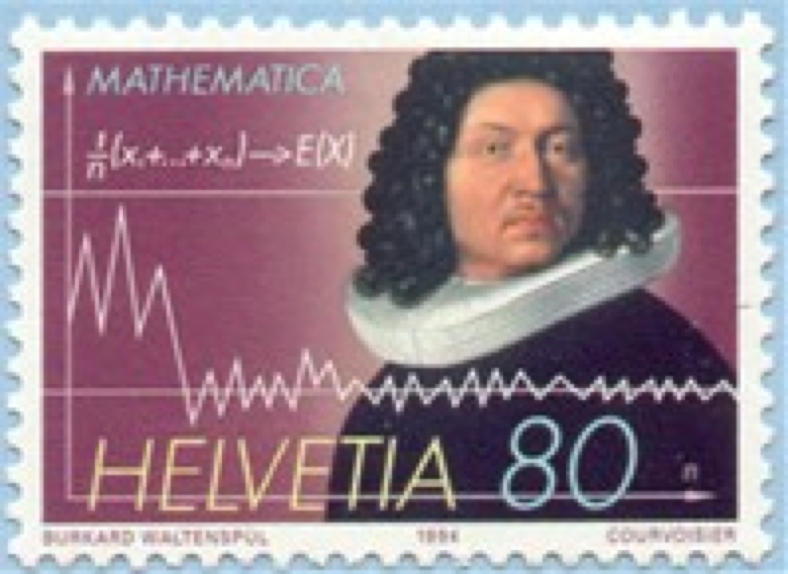
\includegraphics[width=\textwidth]{money/stamp.png}
\caption{纪念邮票}
\end{minipage}
\end{figure}

伯努利家虽然非常有钱,但他不是财主,也没听说过他放贷。但是作为一个出色的数学家
,伯努利在生活中观察到了放贷和利息计算这种行为,并对此进行了细致的研究,最终给
出了复利的终极计算方式,这个终极的计算方式里就包含了$e$。

\begin{figure}[htbp]
\centering
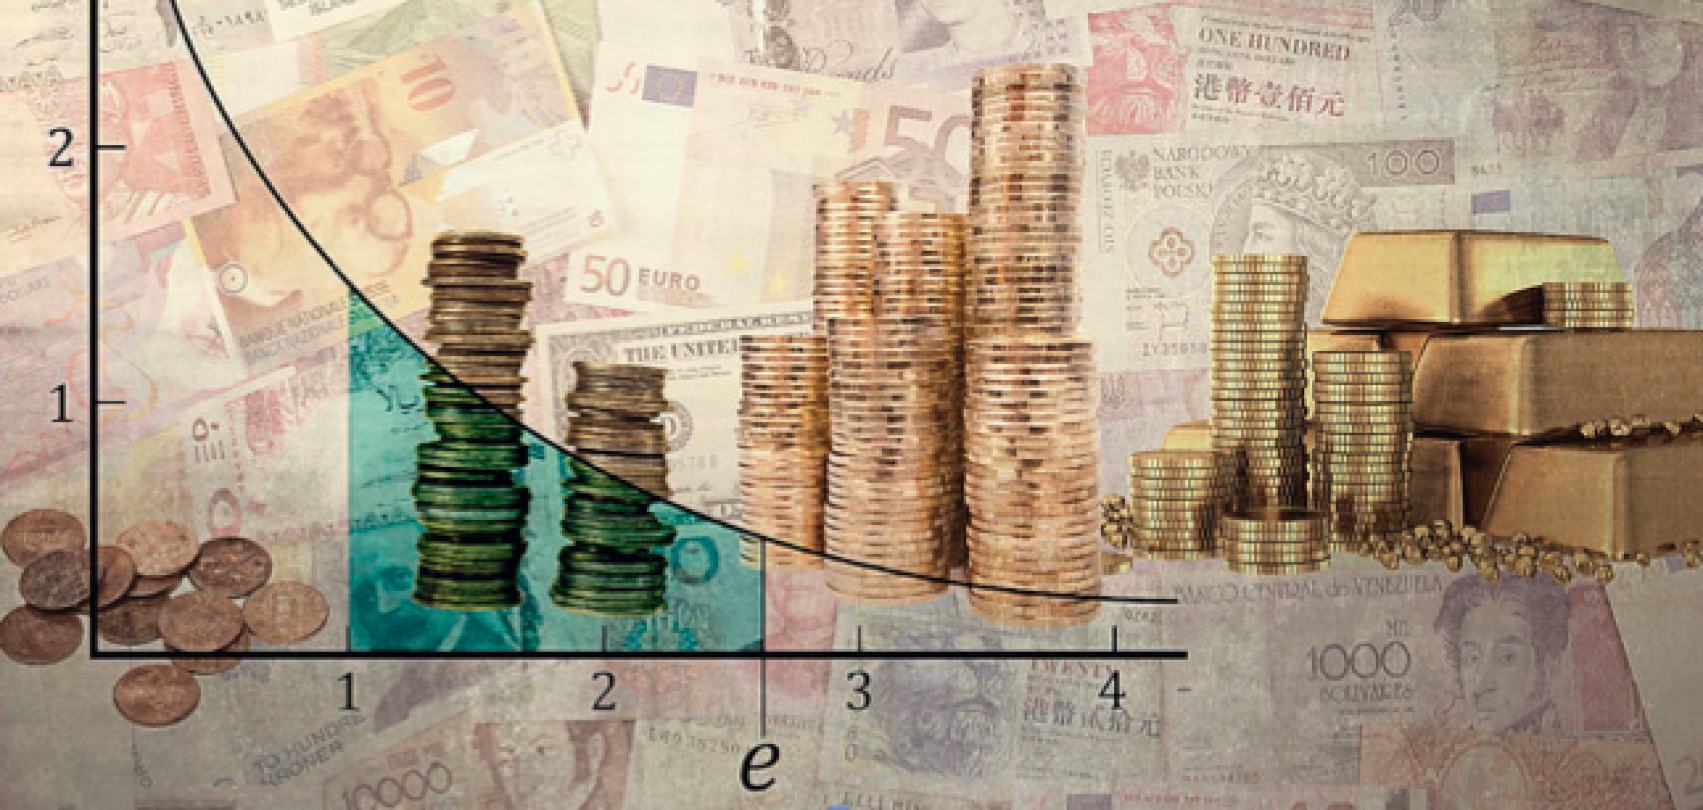
\includegraphics[width=0.9\linewidth]{money/e-interest.png}
\caption{$ e$ 与利息}
\centering
\end{figure}

故事中伯努利老爷算钱的方式其实基本上就是现如今我们银行计算贷款的方式——复利,
也就是大家熟知的利滚利,利息接着产生利息。只是现在银行通常以天为单位来计息,而
且年利率也不会有百分之百那么高,通常是百分之五百分之七。下面这张图显示了年利率
为20\%时,分别按照年(n=1)、季度(n=4)、月份(n=12)和时间无穷细分(n 趋向于
无穷大 )时的复利增长曲线。

\begin{figure}[htbp]
\centering
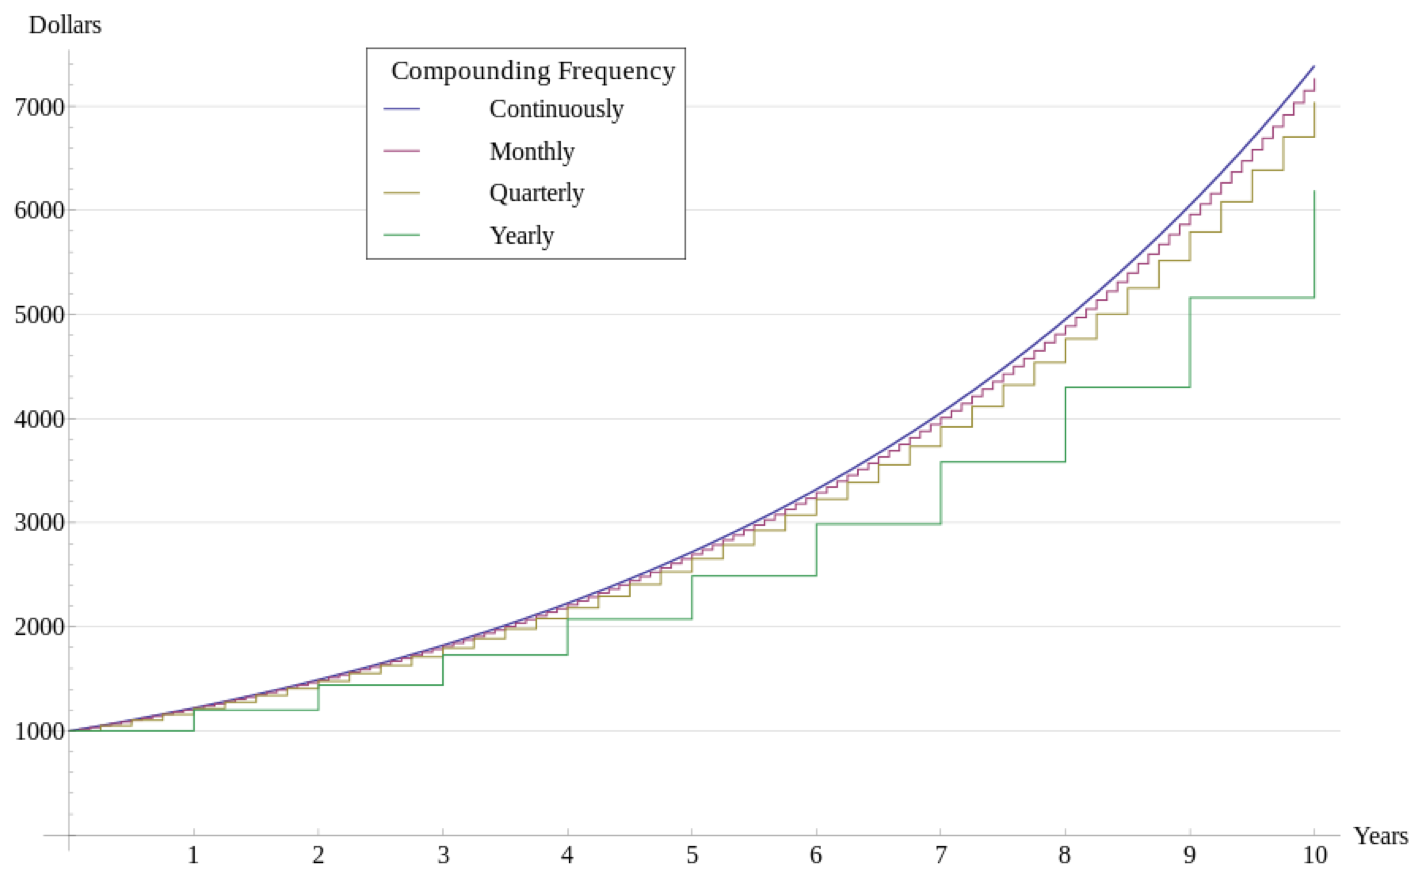
\includegraphics[width=0.9\linewidth]{money/interest.png}
\caption{年利率20\%的复利增长曲线}
\centering
\end{figure}


后告诫大家千万别找数学家借钱,数学家会把每一分该得的钱都计算的清清楚楚,分毫不
差。

\begin{figure}[htbp]
\centering

\includegraphics[width=0.4\linewidth]{money/millionaire2.png}
\caption{数学家}
\centering
\end{figure}


